\vspace{10pt}

{\centering\subsection*{何宇州:桂花}}

\addcontentsline{toc}{subsection}{何宇州:桂花}

\renewcommand{\leftmark}{何宇州:桂花}

\begin{figure}[htbp]

\centering

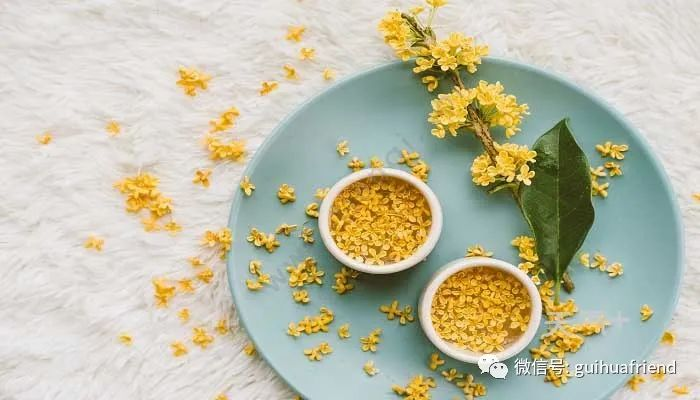
\includegraphics[width = .5\textwidth]{./ch/22.jpg}

\end{figure}



我喜欢的植物有很多,比如兰花、梅花、竹子、菊花……但我最喜欢的是咸宁之花——桂花。

桂花中最具代表性的有金桂、银桂、丹桂、月桂等。

中秋前后百花开尽,桂花才开放。桂花一般有四片花瓣,且小巧玲珑。刚开花时只有仔细的在树之间寻找,才能看到点点黄色,到盛开时,桂花开满了整棵树,一眼望去,黄澄澄,金灿灿,连叶子都快要被遮住了。尤其是黄黄的小花,像雨纷纷落下来的情景,如梦如幻。

我顺手把那几朵鲜嫩的小花骨朵放在手中揉了揉,一下子手就染上淡雅的黄,清新的香味萦绕在我指尖,叫我好不欢喜。

桂花是中国传统十大名花之一。集绿化、美化、香化于一体的观赏与实用兼备的优良园林树种。桂花清可绝尘,浓能远溢 堪称一绝。尤其是中秋时节丛桂怒放,夜静轮圆之际,把酒赏桂,陈香扑鼻,令人神清气爽。



在中国古代的咏花诗词中,咏桂之作的数量也颇为可观,“桂子月中落,天香云外飘。”桂花自古就深受中国人的喜爱,被视为传统名花。

这就是我家乡的桂花,说也说不尽,道也道不完。希望你有机会来细细游赏!





\vspace{10pt}



作者:五(3)班 何宇州



指导老师:刘婷



投稿:2021年5月18日



发表:2021年5月18日






                



\vspace{10pt}

\hline



